\section{Theory}
This section explores some of the depth cues that we use to perceive depth. Furthermore, it explores how \textit{stereopsis} and \textit{binocular disparity} is used to construct stereograms.

\subsection{Oculomotor depth cues}
When trying to focus on objects in close range (< 2m) our eye muscles and lenses react by either convergence or accommodation. \textit{Convergence} means that our eyes turn inward and the lenses take on a rounder shape, when for example trying to focus on objects right in front of the nose. The opposite happens in \textit{accomodation}, which means that the eyes turn more away from each other until they are almost parallel and the lenses will flatten out again. We sense these muscular reactions and are therefore able to determine depth based on them. However, when objects are further away (> 2m) the reaction become so small that we will most likely not notice them\citep[p.~196]{sensationPerception}.

\subsection{Monocular depth cues}
Monocular depth cues only require a single eye, which means that even though we hold a hand over one eye, we are still able to determine depth based on these cues\citep[p.~197]{sensationPerception}

\subsubsection{Partial Occlusion/interposition}
When object partially hide (or occlude) other objects indicating that the hidden object is behind the non-hidden object(See \autoref{fig:partialOcclusion}). This is called \textit{partial occlusion} or \textit{interposition}\citep[p.~197]{sensationPerception}.

\begin{figure}[H]
	\centering
	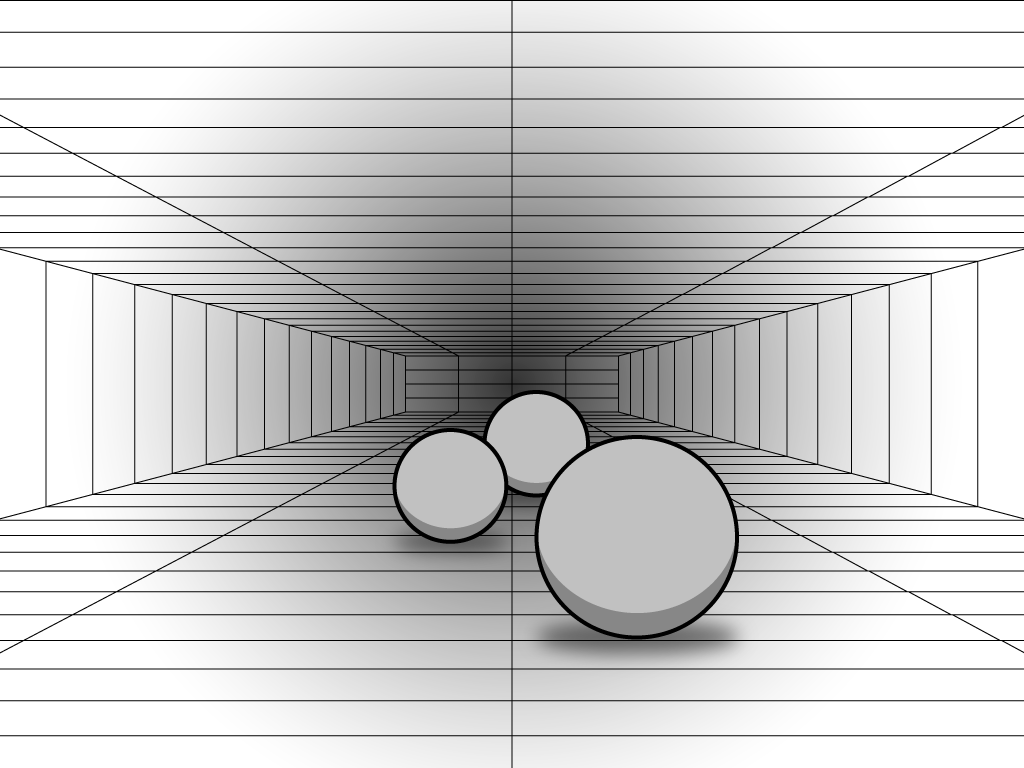
\includegraphics[width=0.8\linewidth]{figure/Analysis/partialOcclusion.png}
	\caption{Partial occlusion (or Interposition) is a monocular cue that identifies objects which overlap others as closer to the viewer.}
	\label{fig:partialOcclusion}
\end{figure}

\subsubsection{Relative height}
In \autoref{fig:relativeHeight} three round objects can be seen. Although, the three objects to be the exact same size, the position of the objects in the image indicate where they are in 3D space. The object positioned higher up is closest to the horizon in the image and will appear to be further away. In this case the object must also be larger than the object positioned lower in the image. This is called \textit{relative height}. The opposite would be true for object hanging from the ceiling\citep[p.~198]{sensationPerception}.

\begin{figure}[H]
	\centering
	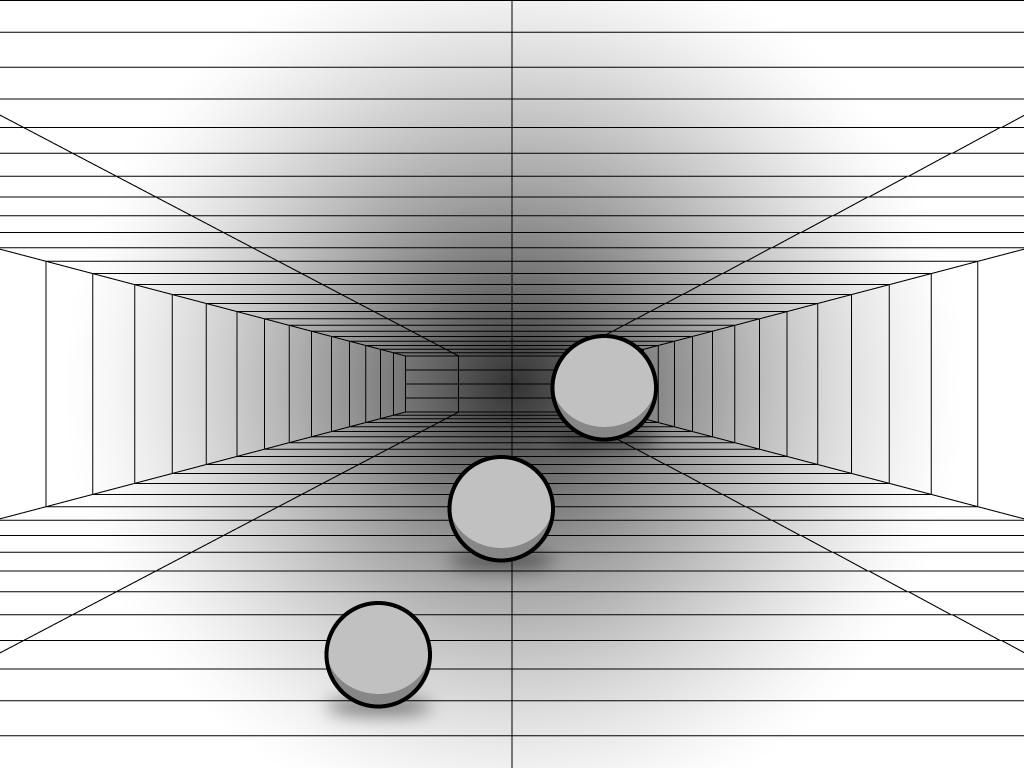
\includegraphics[width=0.8\linewidth]{figure/Analysis/relativeHeight.png}
	\caption{The position of an object with respect to the horizon in this figure indicate the spatial position of the object.}
	\label{fig:relativeHeight}
\end{figure}

\subsubsection{Relative size}
Assuming that the two objects seen in \autoref{fig:relativeSize} have about the same physical size, we are able to place the objects in space based on how large they appear to be in the image. The larger the object appears, the closer it is\citep[p.~200]{sensationPerception}.
\begin{figure}[H]
	\centering
	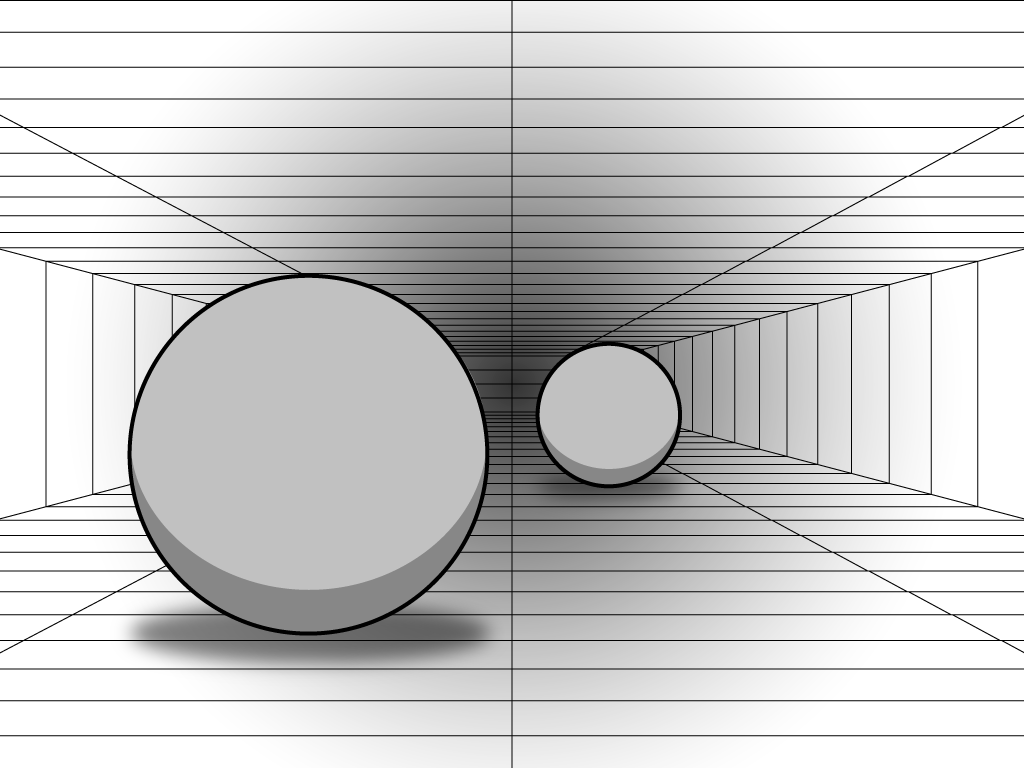
\includegraphics[width=0.8\linewidth]{figure/Analysis/relativeSize.png}
	\caption{Relative size.}
	\label{fig:relativeSize}
\end{figure}

\subsubsection{Linear perspective}
The image in \autoref{fig:linearPerspective} shows what could appear to be a room with a lot of lines. Assuming that the lines on the floor and on the ceiling are parallel, the fact that they seem to converge and get closer together as they move closer to the vanishing point gives the appearance of depth in the \textit{"room"}\citep[p.~201]{sensationPerception}.
\begin{figure}[H]
	\centering
	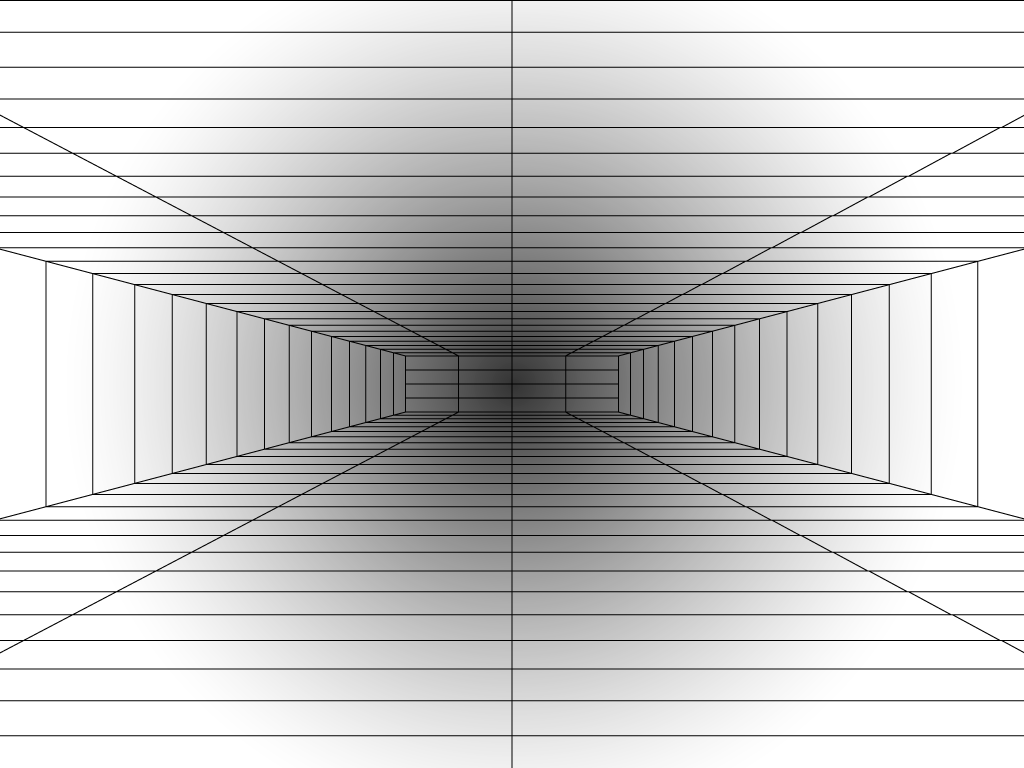
\includegraphics[width=0.8\linewidth]{figure/Analysis/linearPerspective.png}
	\caption{When parallel lines converge as they recede in the distance is called linear perspective.}
	\label{fig:linearPerspective}
\end{figure}

\subsubsection{Atmospheric Perspective}
\autoref{fig:atmosphericPerspective} shows how an objects light information can be distorted by a variety of particles in the air. The object further away appears more hazy and less distinct as the light must travel through a longer distance of air. This is called \textit{atmospheric perspective}\citep[p.~202]{sensationPerception}.
\begin{figure}[H]
	\centering
	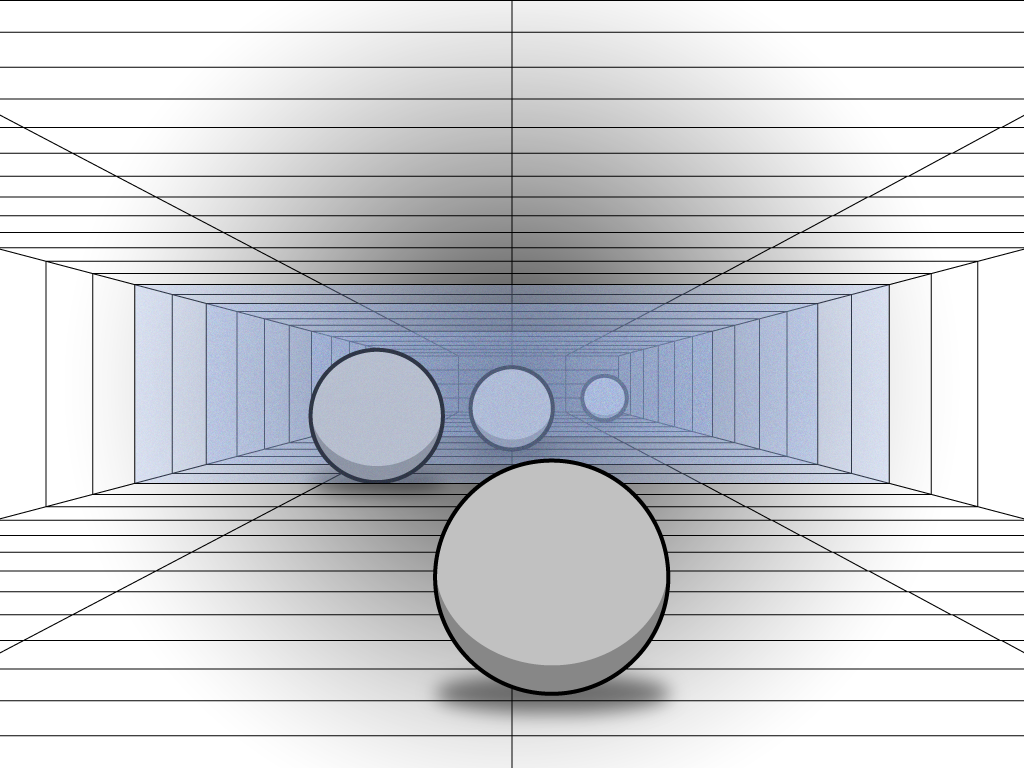
\includegraphics[width=0.8\linewidth]{figure/Analysis/atmosphericPerspective2.png}
	\caption{Atmospheric perspective is a light-based monocular cue. Particles in the air can obscure and distort the retinal information for objects in the distance whereas the objects closest to the viewer appear more clearly.}
	\label{fig:atmosphericPerspective}
\end{figure}

\subsubsection{Shading}
Assume that there is a light source from above in the two images in \autoref{fig:shading}. Based on the \textit{shading} of the objects it appears that the center object of the left image is an indention, while the surrounding objects appear to be raised. The opposite goes for the image on the right\citep[p.~202]{sensationPerception}.
\begin{figure}[H]
	\centering
	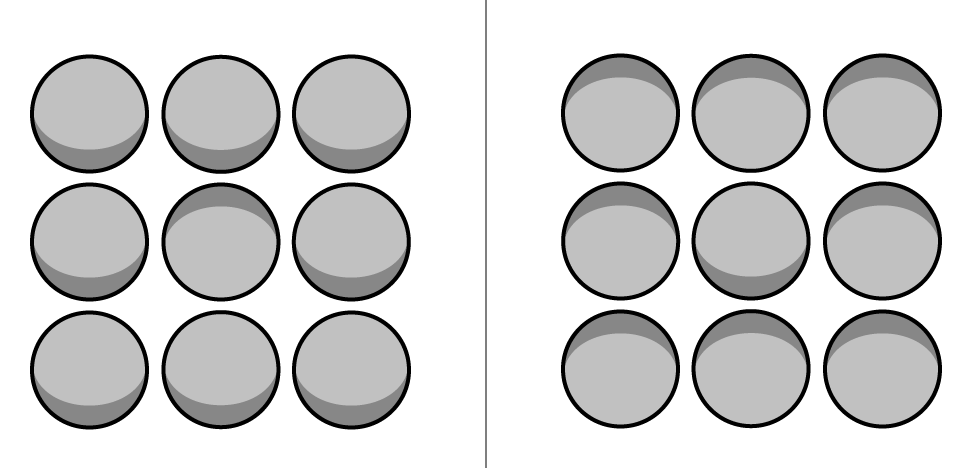
\includegraphics[width=0.8\linewidth]{figure/Analysis/shading.png}
	\caption{Figure showing how depth can be perceived based on illumination and shading of a curved object.}
	\label{fig:shading}
\end{figure}

\subsubsection{Motion parallax}\label{sec:parallax}
\autoref{fig:parallax} shows the movement of three objects in three point in time. We assume that the three round objects move about the same distance from one side of the room to the other at approximately the same speed. It can be seen that an object closer to the observer appears to move a greater distance on the retinal image. This is called \textit{motion parallax} and is one of the dynamic cues\footnote{Dynamic cues require movement of either the viewer or the object in order to determine the spatial position of objects\citep{sensationPerception}.}\citep[p.~204]{sensationPerception}.
\begin{figure}[H]
	\centering
	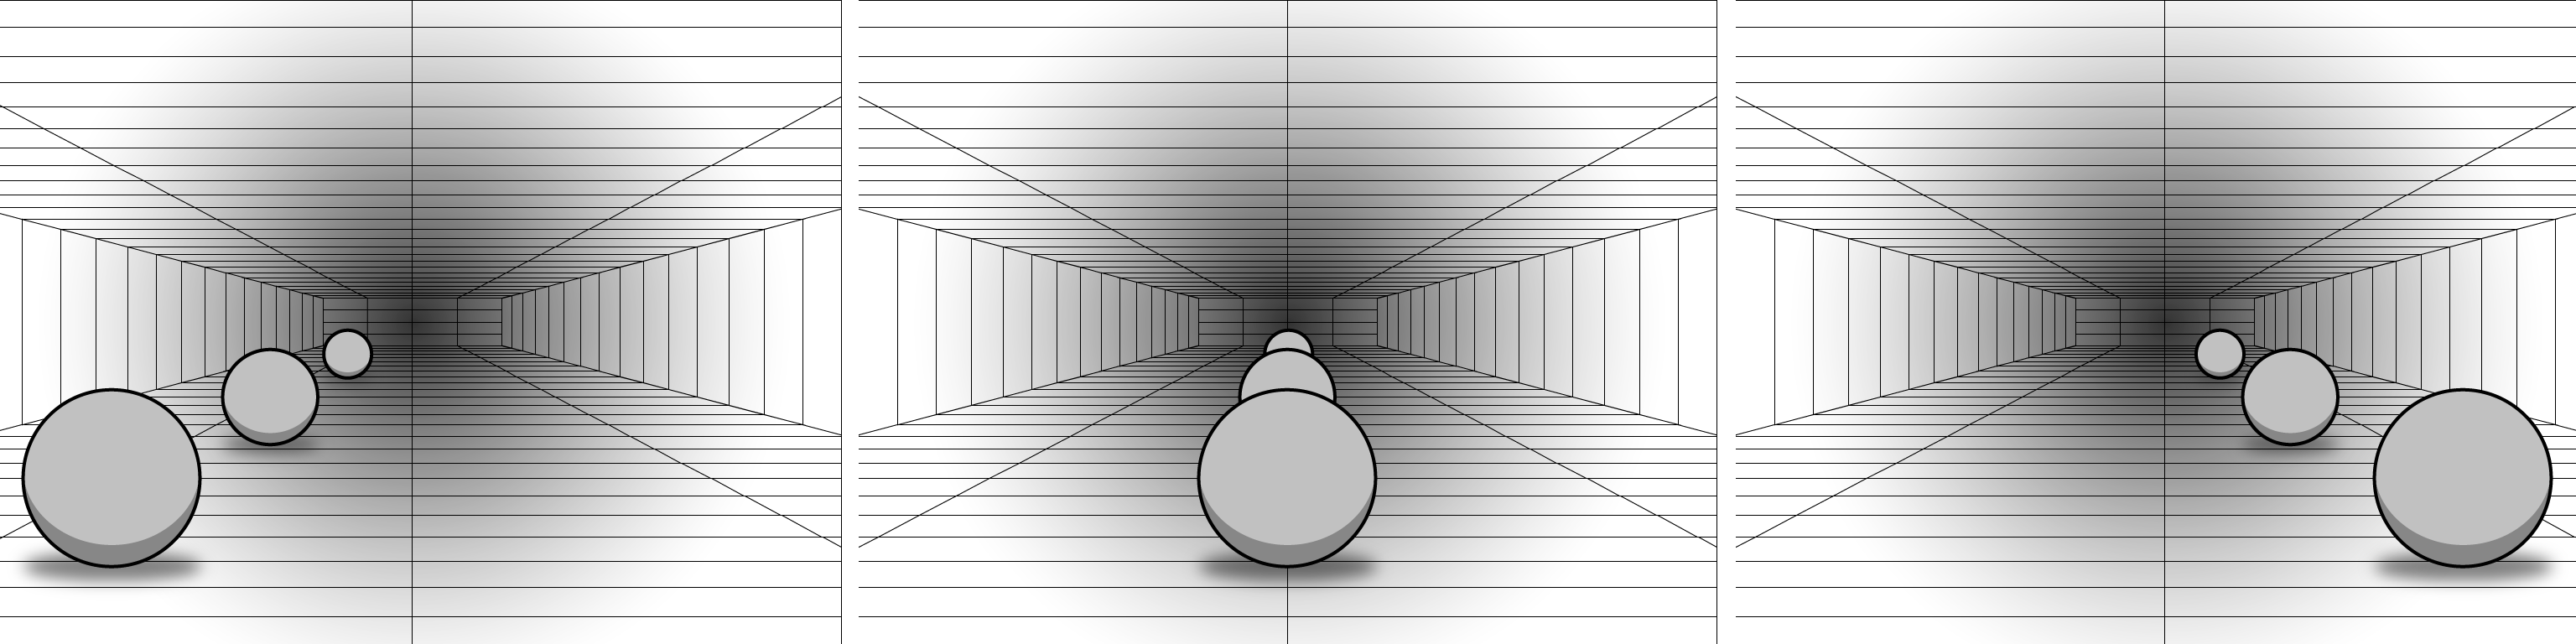
\includegraphics[width=1\linewidth]{figure/Analysis/parallax.png}
	\caption{Motion parallax}
	\label{fig:parallax}
\end{figure}

\subsubsection{Deletion and accretion}
Another one of the dynamic monocular depth cues, which is also related to occlusion(See \autoref{fig:partialOcclusion}), is called \textit{deletion and accretion}. If we imagine that the round object in \autoref{fig:deletionAccretion} is the same object at different times moving from the left to the right, deletion occurs when the object is moving behind another object(the box) making it partially occluded and accretion happens when the object reappears on the right side of the box and is gradually de-occluded\citep[p.~207]{sensationPerception}.
\begin{figure}[H]
	\centering
	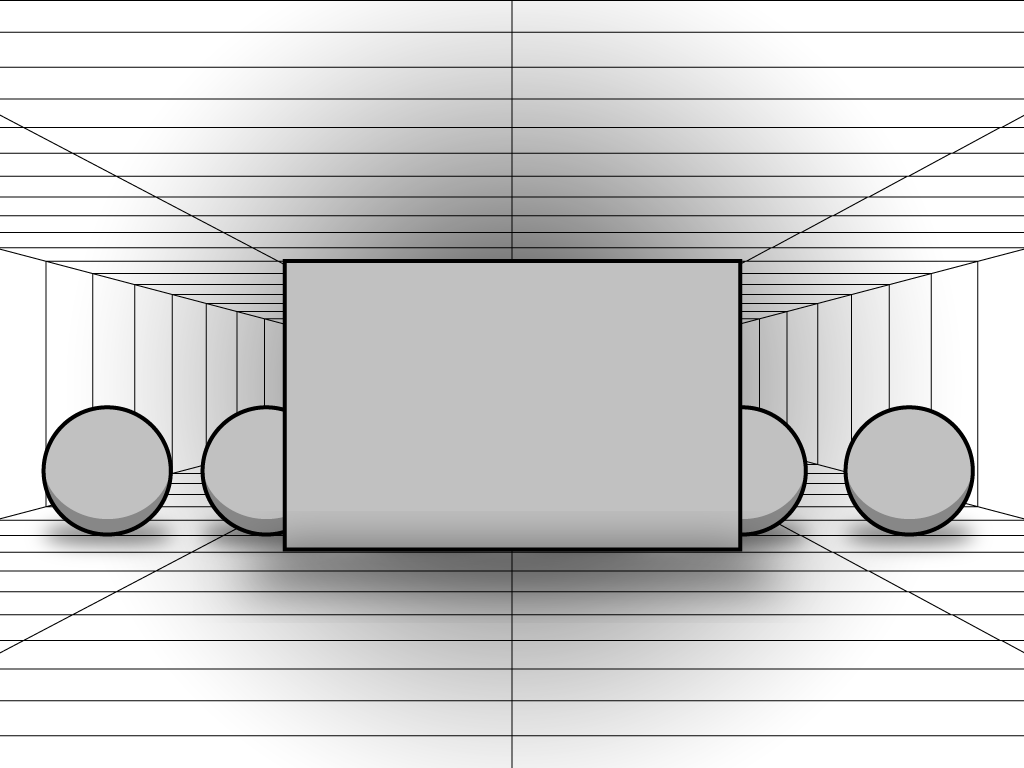
\includegraphics[width=0.8\linewidth]{figure/Analysis/deletionAccretion.png}
	\caption{Deletion and accretion.}
	\label{fig:deletionAccretion}
\end{figure}


\subsection{Binocular depth cues}\label{sec:binocularDepthCues}
A depth cue that requires the use of both eyes is called Binocular depth cues. As seen in \autoref{fig:depthCues} this category only contains one cue, which is \textit{Binocular disparity}. Due to our eyes being positioned horizontally different the 2D retinal images from both eyes will be slightly different as seen in \autoref{fig:stereoscopicVision}. Binocular disparity is the difference in position of the object being looked at with each eye\citep[p.~208]{sensationPerception}. The differences in the two 2D images from both eyes are processed in our brain to makes us perceive the surrounding 3D space. This is a powerful depth cue for species with front facing eyes\citep{seeingInThreeDimensions}. Binocular disparity is also used in Head-mounted displays(HMD)\citep{hmdCues}.
\begin{figure}[H]
	\centering
	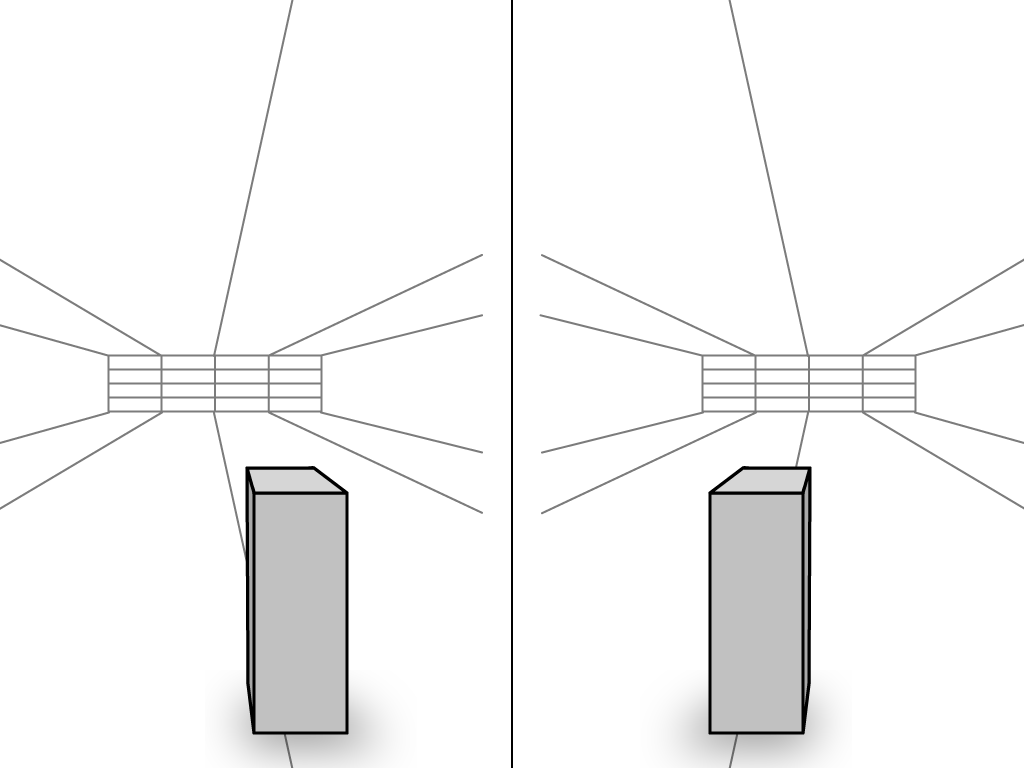
\includegraphics[width=0.8\linewidth]{figure/Analysis/stereoScopicVision.png}
	\caption{Figure illustrating a difference in each eyes' retinal image when looking at an object. The left image corresponds to the left eyes view and the right image corresponds to the right eyes view.}
	\label{fig:stereoscopicVision}
\end{figure}


\subsection{Stereopsis and binocular disparity in stereograms}\label{sec:stereograms}
%Under what conditions do the various cues operate? In particular, explain what is meant by "stereopsis" and "binocular disparity" and how these are used in the construction of stereograms and autostereograms.
The term \textit{stereopsis} (or stereoscopic depth perception) refers to the depth perception perceived through \textit{binocular disparity}\citep{sensationPerception,seeingInThreeDimensions}. It has been showed that binocular disparity alone can give make us perceive depth\citep{autostereograms}. Stereograms were invented by Charles Wheatstone as a part of his research in stereopsis. It is, when a set of images, similiarly to the two images shown in \autoref{fig:stereoscopicVision}, can, if viewed through a stereoscope, make a scene appear to be in 3D, provided that the two viewing angles were approximately 6cm apart, as if it were viewed by two eyes\citep[p.~212]{sensationPerception}. An autostereogram, however, is a single image stereogram containing a repeated pattern, that, if looked at in a certain way, can make parts of the pattern \textit{pop out} give an illusion of depth and reveal objects or shapes \textit{"hidden"} within the pattern.\citep{autostereograms}. The image in \autoref{fig:autostereogramExample} is an example of such an autostereogram.

\begin{figure}[H]
	\centering
	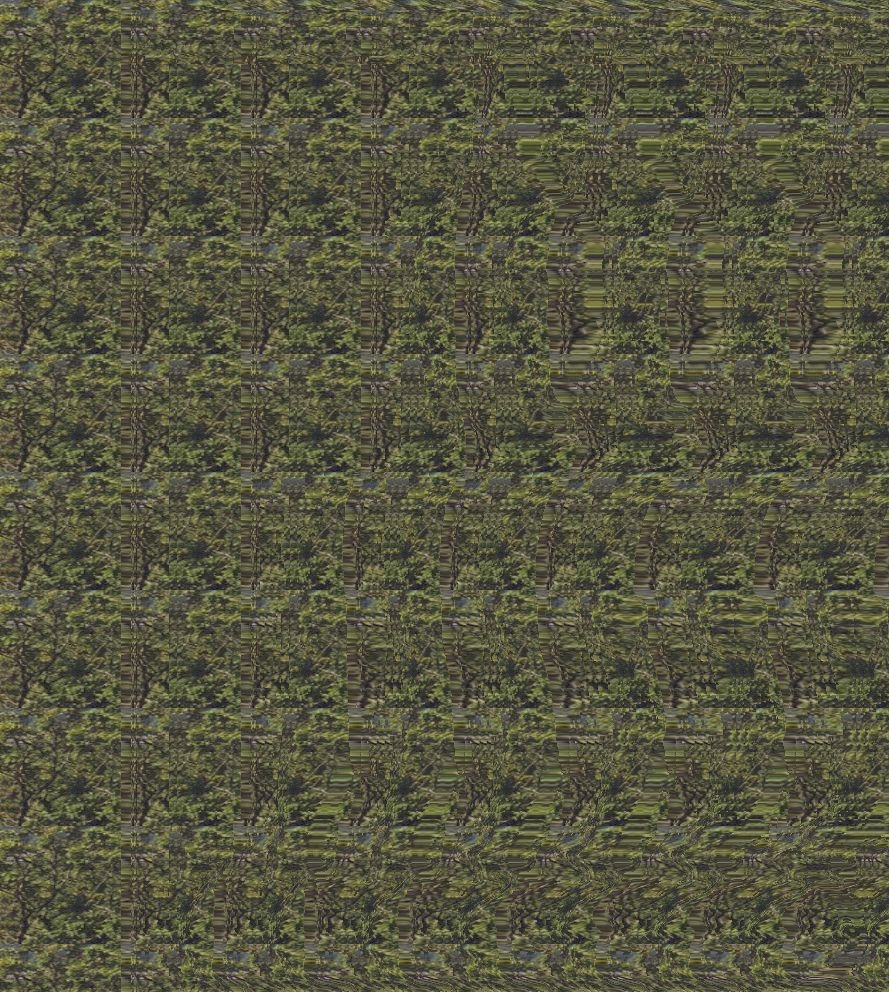
\includegraphics[width=1\linewidth]{figure/Analysis/autostereogram.jpg}
	\caption{Example of an autostereogram example containing a buddha shaped figure.(Created using \href{http://www.easystereogrambuilder.com/3d-stereogram-maker.aspx}{\color{blue}Easy Stereogram Builder})}
	\label{fig:autostereogramExample}
\end{figure}

The repetition of the pattern is constructed in such a way that the parts of the pattern repeat themselves in different length intervals or with different lengths between them. When viewed through two eyes, and if the viewers focal point is either in front of- or behind the image plane, two parts will fuse with each other and become one, making different parts of the image pattern appear to float on different depths\citep{autostereogramNguyen}. \autoref{fig:autostereogram} is a simple illustration of how shorter repetition distances make object seem closer to the viewer(green) and how longer distances will make the parts seem further away(blue). 

\begin{figure}[H]
	\centering
	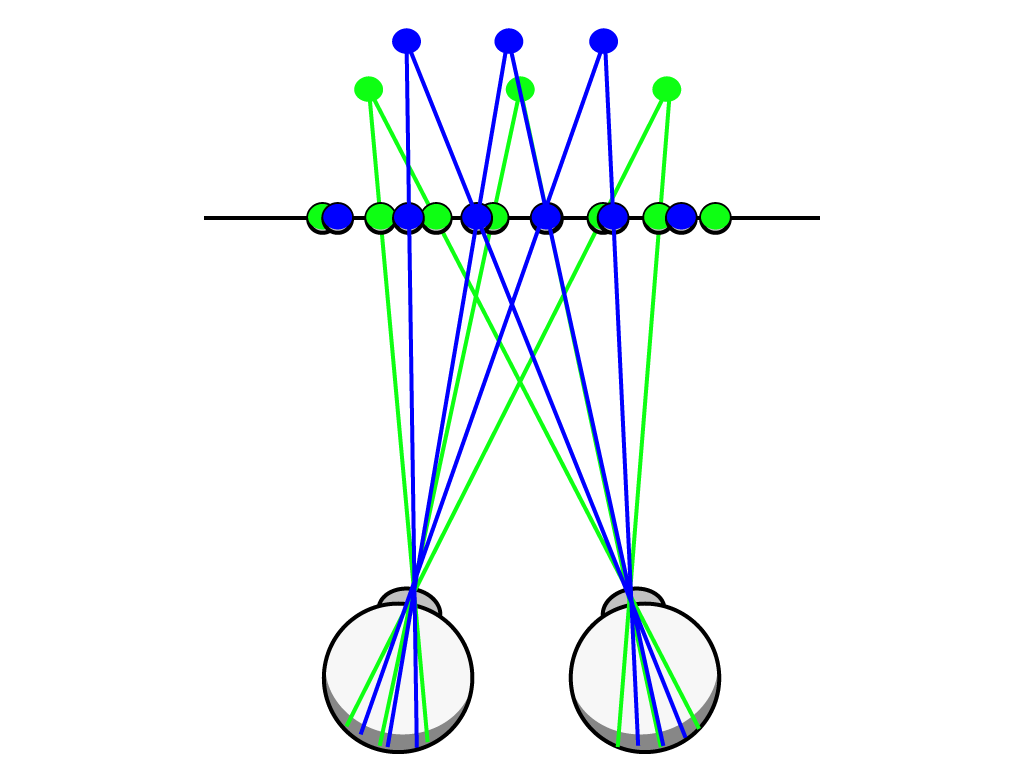
\includegraphics[width=0.8\linewidth]{figure/Analysis/autoStereogram.png}
	\caption{Figure showing how dots with different distances between them in a repeating pattern, through the use of both eyes, can make parts appear on different depths, when the focal point is not directly on the image plane.}
	\label{fig:autostereogram}
\end{figure}

\section{Discussion}
This section discusses the topics from the previous section. It also explores various ways of how depth perception is integrated in modern digital media technology.

	\subsection{Visual impairments}
	In all of the examples throughout this paper, it is assumed that the viewer has the sight of an normal person, meaning that visual impairments have not been considered in any way. An example where this might be a relevant issue is binocular disparity, which is described in \autoref{sec:binocularDepthCues}. If a viewer does not have two functioning eyes, that is required to perceive depth through stereoscopic vision, he/she must rely on other depth cues.

	\subsection{Parallax scrolling}
	A lot of the screen-based electronic devices available today use depth cues in order to give the appearance of depth on the screen, which is essentially a 2D image. An example of this is motion parallax, which is described in \autoref{sec:parallax}. This is popular web design technique that makes objects on the screen move at different speeds as a user scrolls through a website, giving a 3D effect\citep{parallaxWeb}. Apple also introduced a parallax effect to the homescreen of iPhones and iPads with the release of iOS 7, which made icons appear to levitate above the background image as the device was moved\citep{ios7}.

	\subsection{Virtual reality}
	Virtual reality is another application that make use of depth cues. As previously mentioned in \autoref{sec:binocularDepthCues} HMDs use binocular disparity to place a user within an immersive virtual 3D environment that can be explored and interacted with\citep{hmdCues}. However, other cues are also applied in virtual environments such as Shadows and perspective. Virtual reality has become increasingly popular for different types of applications like games, simulations, training and research, although if the conditions are not optimal; using a HMD can cause discomfort, strain the eyes and induce motion sickness possibly due to sensory conflicts\citep{hmdCues,motionSickness}.

	\subsection{Autostereograms as an artform}
	Autostereograms became a popular form of art with the release of the book series \textit{"Magic eye"}\citep{autostereograms}, and they have since then also been used in video form as well. An example of this is a music video for the song \href{https://www.youtube.com/watch?v=2AKtp3XHn38}{\color{blue}\textit{"Black is good"} by Young Rival}.

	\subsection{Microsoft Kinect}
	Modern technology is also allowing cameras and sensors to measure depth and reconstruct 3D scenes. Some of these use a process called Time-of-flight. This is a process where optical devices emit light rays into a 3D space and measure the time it takes the light rays to be reflected back to the sensor(longer time = longer distance and vice versa), and thereby are able to generate depth maps of the scene. An example of these devices is the Microsoft Kinect 2\citep{tof}. The first Microsoft Kinect used a different approach for depth measurement which is triangulation. The device emits a speckle pattern of infrared dots onto the scene and by comparing the this pattern to a baseline pattern stored in memory it is able to detect changes in the environment and generate a depth map\citep{pointCloud}.
	

\section{Summary and Conclusion}
This paper has described some of the depth cues, that we use in order to visually perceive depth. However, it did not explore echolocation as a tool of perceiving depth. An example of species that use auditory stimuli to pinpoint objects in 3D space are bats\citep[p.~381]{sensationPerception}. We use visual depth perception in our everyday lives to navigate the three dimensional world around us, driving in traffic and estimating distances to objects. We also use it as entertainment in a media technology in a variety of ways, for example Virtual Reality.

